\documentclass[journal, a4paper]{IEEEtran}

\usepackage{cite} 

\usepackage{graphicx}   
%\usepackage{psfrag}    
%\usepackage{subfigure}
\usepackage{url}        
%\usepackage{stfloats}  
\usepackage{amsmath}    
%\interdisplaylinepenalty=2500
                      
\usepackage{wasysym}

\usepackage{hyperref}

% Your document starts here!
\begin{document}

	\title{Fabrication and testing of 2D and 3D iDEP geometries}
	\author{Malcolm Horal -- F10, XYZ XYZ --XYZ
	\thanks{Malcolm Horal: ine11mho@student.lu.se} \thanks{XYZ XYZ: XYZ@XYZ.XYZ}}
    
	\markboth{Lund University}{}
	\maketitle

\begin{abstract}
Dieclectrophoresis (DEP) is a well-established technique to separate particles from their surrounding medium. In this report insulator-based dielectrophoresis (iDEP) provides a novel, promising approach, achieving an electric field gradient by building insulating “obstacles” into the micro channels and thus trapping or focusing particles. Micro channels are simulated, fabricated and tested for both 2D and 3D geometries with different fluids and particles. It is qualitatively observed that fabrication, simulation and trapping works in all tested dimensions.
\end{abstract}

\section{Introduction}\label{sec:intro}
\PARstart{M}{icrofluidics} is today increasing its influence over a wide range of fields; the pharmaceutical, clinical, biochemical and environmental. It is continuously proving its relevance as an appropriate tool for a variety of purposes, such as screening, separating, sorting or trapping fluids and particles. Miniaturization of analytical systems offer numerous advantages, such as reduced sample and reagent consumption, shorter response and analysis time, higher throughput, automation, greater sensitivity, mobility and last but not least, low cost \cite{mark2010,srivastava2011}. The field is developing rapidly and new techniques and niches are constantly being exploited.

Dieclectrophoresis (DEP) is a well-established technique to separate particles from their surrounding medium. It is one of the most efficient techniques and widely used for separation of proteins, DNA, virus and bacteria. Among some of its advantages are the facts that it is label free, has a high selectivity and sensitivity and is easily integrated with other chip devices \cite{cheri2014,martinez2009,srivastava2011}.

DEP is an electrokinetic transport mechanism produced from the polarization that arises when microparticles are exposed to a non-uniform electric field (AC or DC).  Traditionally, the non-uniformity of the electric filed was obtained by utilizing AC voltage to an array of microelectrodes embedded in the microchannel network (electrode based DEP, eDEP). Despite obtaining high electric field gradients at low voltages, major drawbacks with this method persist: the complex and expensive fabrication process (thin film deposition), functionality failure over time of the metal electrodes due to electrolysis, and limited compatibility with biological samples, due to Joule heating effects and adverse reactions with the electrodes \cite{Braff:12,cheri2014}. Thus, creating the DEP-force with other means would be desirable. Here insulator-based dielectrophoresis (iDEP) provides a new, promising approach, carrying out DEP in an alternative manner; achieving an electric field gradient by building insulating  “obstacles” into the channel. Devices employing the iDEP technique have already been used in biological applications such as cell sorting, to determine cell concentration and to enhance DNA hybridization \cite{Braff:12}.

The major objective of this project is to investigate the iDEP technique under different conditions in a microchannel. By varying the constriction ratio of the channel, changing its dimensions in both 2D and 3D, the aim is to conclude to what extent this affects the channels’ ability to focus and trap particles. And, primarily, if we at 3D constrictions can get trapping at lower voltages than in the channels with 2D constrictions.


\section{Dep \& Idep}
In order to overcome the need for numerous electrodes and still create a non-uniform electric field, an iDEP construction utilizes only two electrodes, placed at each end (inlet and outlet) of the microchannel.  Instead of an array of electrodes, the channel contains an array of insulating structures. When an electric potential is applied over the channel, the presence of the insulating structures creates regions with varying electric field strength– which is necessary for DEP to occur \cite{martinez2009}.  Around the insulating structures, particles will be either trapped or focused. 
The physical background of the iDEP phenomena is that the electric field gradient, generated around the obstacles within a channel, polarizes the particle and the dielectric medium. This leads to unequal forces acting on the particle, resulting in a net force, which is the DEP force $\mathbf{F}_{DEP}$ described below \cite{pethig1997}. 

\begin{equation}\label{eq:idepForce}
\mathbf{F}_{DEP}=2\pi\varepsilon _{m}a^{3}\kappa \boldsymbol{\Delta }\left (\boldsymbol{E}\boldsymbol{\cdot \boldsymbol{E}}  \right )
\end{equation}

The force thus depeneds on particle size, permittivity of the medium and the electric field applied. $\kappa$ is the Clausius-Mossotti factor, in a DC field a function of the particles and medium conductivity, and the sign of which determines if the DEP-force is positive or negative. In a DC field, the complex permittivity is dominated by the conductivity of the particle, and the Clausius-Mossotti factor can hence be expressed as in~\eqref{eq:klasse}. Positive DEP (p-DEP) attracts particles towards regions of higher electric field strength, whereas n-DEP causes a repulsive movement of particles away from these regions \cite{cheri2014}.

\begin{equation}\label{eq:klasse}
\kappa =\frac{\sigma _{p}-\sigma _{m}}{\sigma _{p}+2\sigma _{m}}
\end{equation}

Electroosmosis from an applied DC voltage drives the bulk flow of the fluid within the channel, which eliminates the need for an external pump and further simplifies the design of the device \cite{Braff:12}. When the particle motion is balanced due to the bulk fluid flow, trapping occurs. The motion of the particles due to the DEP-force is described below in equation~\eqref{eq:vDEP}. The particle motion thus depends on its dielectrophoretic mobility $\mu _{DEP}$, and the applied electric field $\boldsymbol{E}$. The dielectrophoretic mobility can also further be expressed as a function of the previously mentioned Clausius-Mossotti factor $\kappa$, particle radius $a$, permittivity $\varepsilon _{m}$ and medium viscosity $\eta$.

\begin{equation}\label{eq:vDEP}
\begin{matrix}
\boldsymbol{v}_{DEP}=\mu _{DEP}\boldsymbol{\Delta \left ( \boldsymbol{E}\times \boldsymbol{E} \right )}\\ 
\mu _{DEP}=\frac{\varepsilon _{m}\kappa a^{2}}{3\eta } 
\end{matrix}
\end{equation}

A trapping parameter $\alpha _{max}$ is defined \eqref{eq:alfa}, depending on the particle mobilites arising from dielectrophoresis, electroosmosis and electrophoresis, as well as on the channel's dimensions (length $L$, width $w$), the constriction ratio $\chi$ and the applied voltage $V_{0}$.  Trapping occurs when $\alpha$ is larger than 1. The sensitivity of an iDEP device can thus be defined as the change in trapping strength for a given change in applied voltage \cite{Braff:12}.

\begin{equation}\label{eq:alfa}
\alpha _{max}\approx \frac{\mu _{DEP}}{\mu _{EO}+\mu _{EP}}\frac{V_{0}\chi }{Lw}
\end{equation}

As equation~\eqref{eq:alfa} clearly depicts, there is a strong dependency between the constriction ratio $\chi$ and the sensitivity of the device. A high constriction ratio can also compensate for applying lower voltages, yet yielding the same level of trapping. Previous mentioned studies have reported differences between when a constricted region of the channel has been constricted in two or three dimensions, so called 2DiDEP and 3DiDEP. By constricting a channel in two dimensions rather than one, the constriction ratio can be made an order of magnitude larger, thus allowing particles to be trapped at average electric fields one order of magnitude lower. Operating at lower voltages minimizes \textit{Joule heating} effects, making iDEP more applicable for biological applications \cite{Braff:12}. Additionally, fouling effects is not as detrimental to an iDEP system as to an eDEP, since it does not impede the function of the system. This also makes iDEP more suitable for biological applications. Another advantage with the iDEP technique is that the channels can be fabricated from cheap materials such as plastics, increasing their potential for high throughput applications \cite{martinez2009}.

\section{Method}\label{sec:method}

\subsection{FEM simulations}
By simulating the experimental setup in COMSOL Multiphysics\textsuperscript{\textregistered} the electric field and electroosmotic flow can be studied separately to support the experimental data. Due to the limits of the academic license of the software, which prohibited the use of the micifluidics module, only the electric field was simulated. An electric potential between the inlet (leftmost wall) and outlet (rightmost wall) was introduced and all other walls of the the channel was set to be isolated. The properties of the channel medium was chosen to be equal that of water.

\subsection{Fabrication}
The main focus of the experiments was to compare the iDEP forces generated by 2D and 3D geometries, respectively, by investigating how the magnitude of the constriction ratio affects the generation of an iDEP force. To do that five different micro channels were fabricated.

In the 2D case, three different channels with main channels of different widths, but with equal dimensions of the constricted section, were compared. The constricted part of the channel have a constricted width of 100 $\mu$m, while the depth was maintained and equal to the depth of the main channel (100 $\mu$m). This constitutes the 2D constriction ratio, thereby creating different operating conditions for each channel. Both the total volume of fluid in the main channel as well as the constriction ratio were varied for each channel, potentially providing information regarding the impact these parameters have on the iDEP phenomena. These dimensions create a constriction ratio of 5 for channel 1, 10 for channel 2, (which has been proven sufficient for trapping of particles in previous iDEP experiments \cite{Braff:12}), and channel 3 had a ratio of 20. The fabrication process placed certain constraints on how small dimensions could be created. The channel dimensions for each of the three channels can be seen in~\ref{tab:dim}.

By keeping the constricted part consistent and vary the depth of the main channel, the ratio could be increased further and the constriction depth and channel depth relation would be evaluated for two more channel depths: 200 and 400 $\mu$m, creating constriction ratios of 20 resp. 40. Other dimensions remained identical to those of channel 2. A summary of all dimensions is seen in table~\ref{tab:dim}.

\begin{table}[!hbt]
\centering
\caption{Main dimensions (left) \& constriction dimensions (right) for 2D \& 3D channels.}
\label{tab:dim}
\begin{tabular}{c|ccc|ccc}
\textbf{Chan}  & \textbf{Width} & \textbf{Depth} & \textbf{Length} & \textbf{con. W} & \textbf{con. D} & \textbf{con. L} \\ \hline
1 [mm]& 0.5              & 0.1            & 10              & 0.1            & 0.1            & 0.5             \\
2 [mm]& 1            & 0.1            & 10              & 0.1            & 0.1            & 0.5             \\
3 [mm]& 2              & 0.1            & 10              & 0.1            & 0.1            & 0.5  \\ \hline
4 [mm]& 1            & 0.2            & 10              & 0.1            & 0.1            & 0.5             \\   
5 [mm]& 1            & 0.4            & 10              & 0.1            & 0.1            & 0.5            
\end{tabular}
\end{table}

The designs of the channels were created in Fusion360\textsuperscript{\textregistered} and can be seen in Fig.~\ref{fig:CAD} and Fig.~\ref{fig:CAD3D}.

Duplicates of each channel design were created. All 10 channels were micro milled on a 2 mm thick PMMA sheet with a surface dimensions of 25 by 75 mm. The whole structure was cleaned with soap, water and acoustics. The structure were then exposed to a UV/ozone treatment to further clean the structure and activate the surface prior to being thermally bonded with a lid at 110$^{\circ}$ C. Tubes of stainless steel made from cut off syringe needles were carefully attached at the ends of the channels to serve as inlets/outlets. The final result can be seen in Fig.~\ref{fig:chip}.

\begin{figure}
	\begin{center}
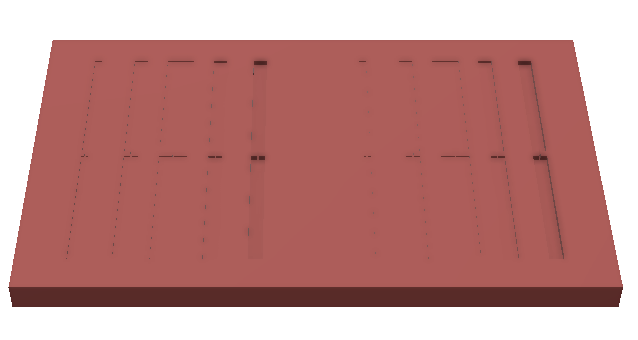
\includegraphics[width=0.5\textwidth]{cad3De.png}
		\caption{\label{fig:CAD3D} 3D model of all channels on a chip created in Fusion360\textsuperscript{\textregistered}. Channels numbers in sequence from left to right, twice: 1, 2, 3, 4, 5, etc.}
    \end{center}
\end{figure}

\begin{figure}
\begin{center}
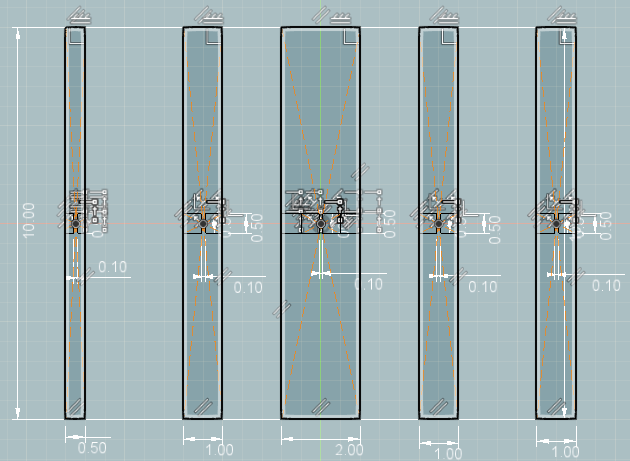
\includegraphics[width=0.5\textwidth]{sketch2d.png}
		\caption{\label{fig:CAD} 2D sketch of channels 1 through 5 intended for testing iDEP.}
        \end{center}
\end{figure}

\begin{figure}
	\begin{center}
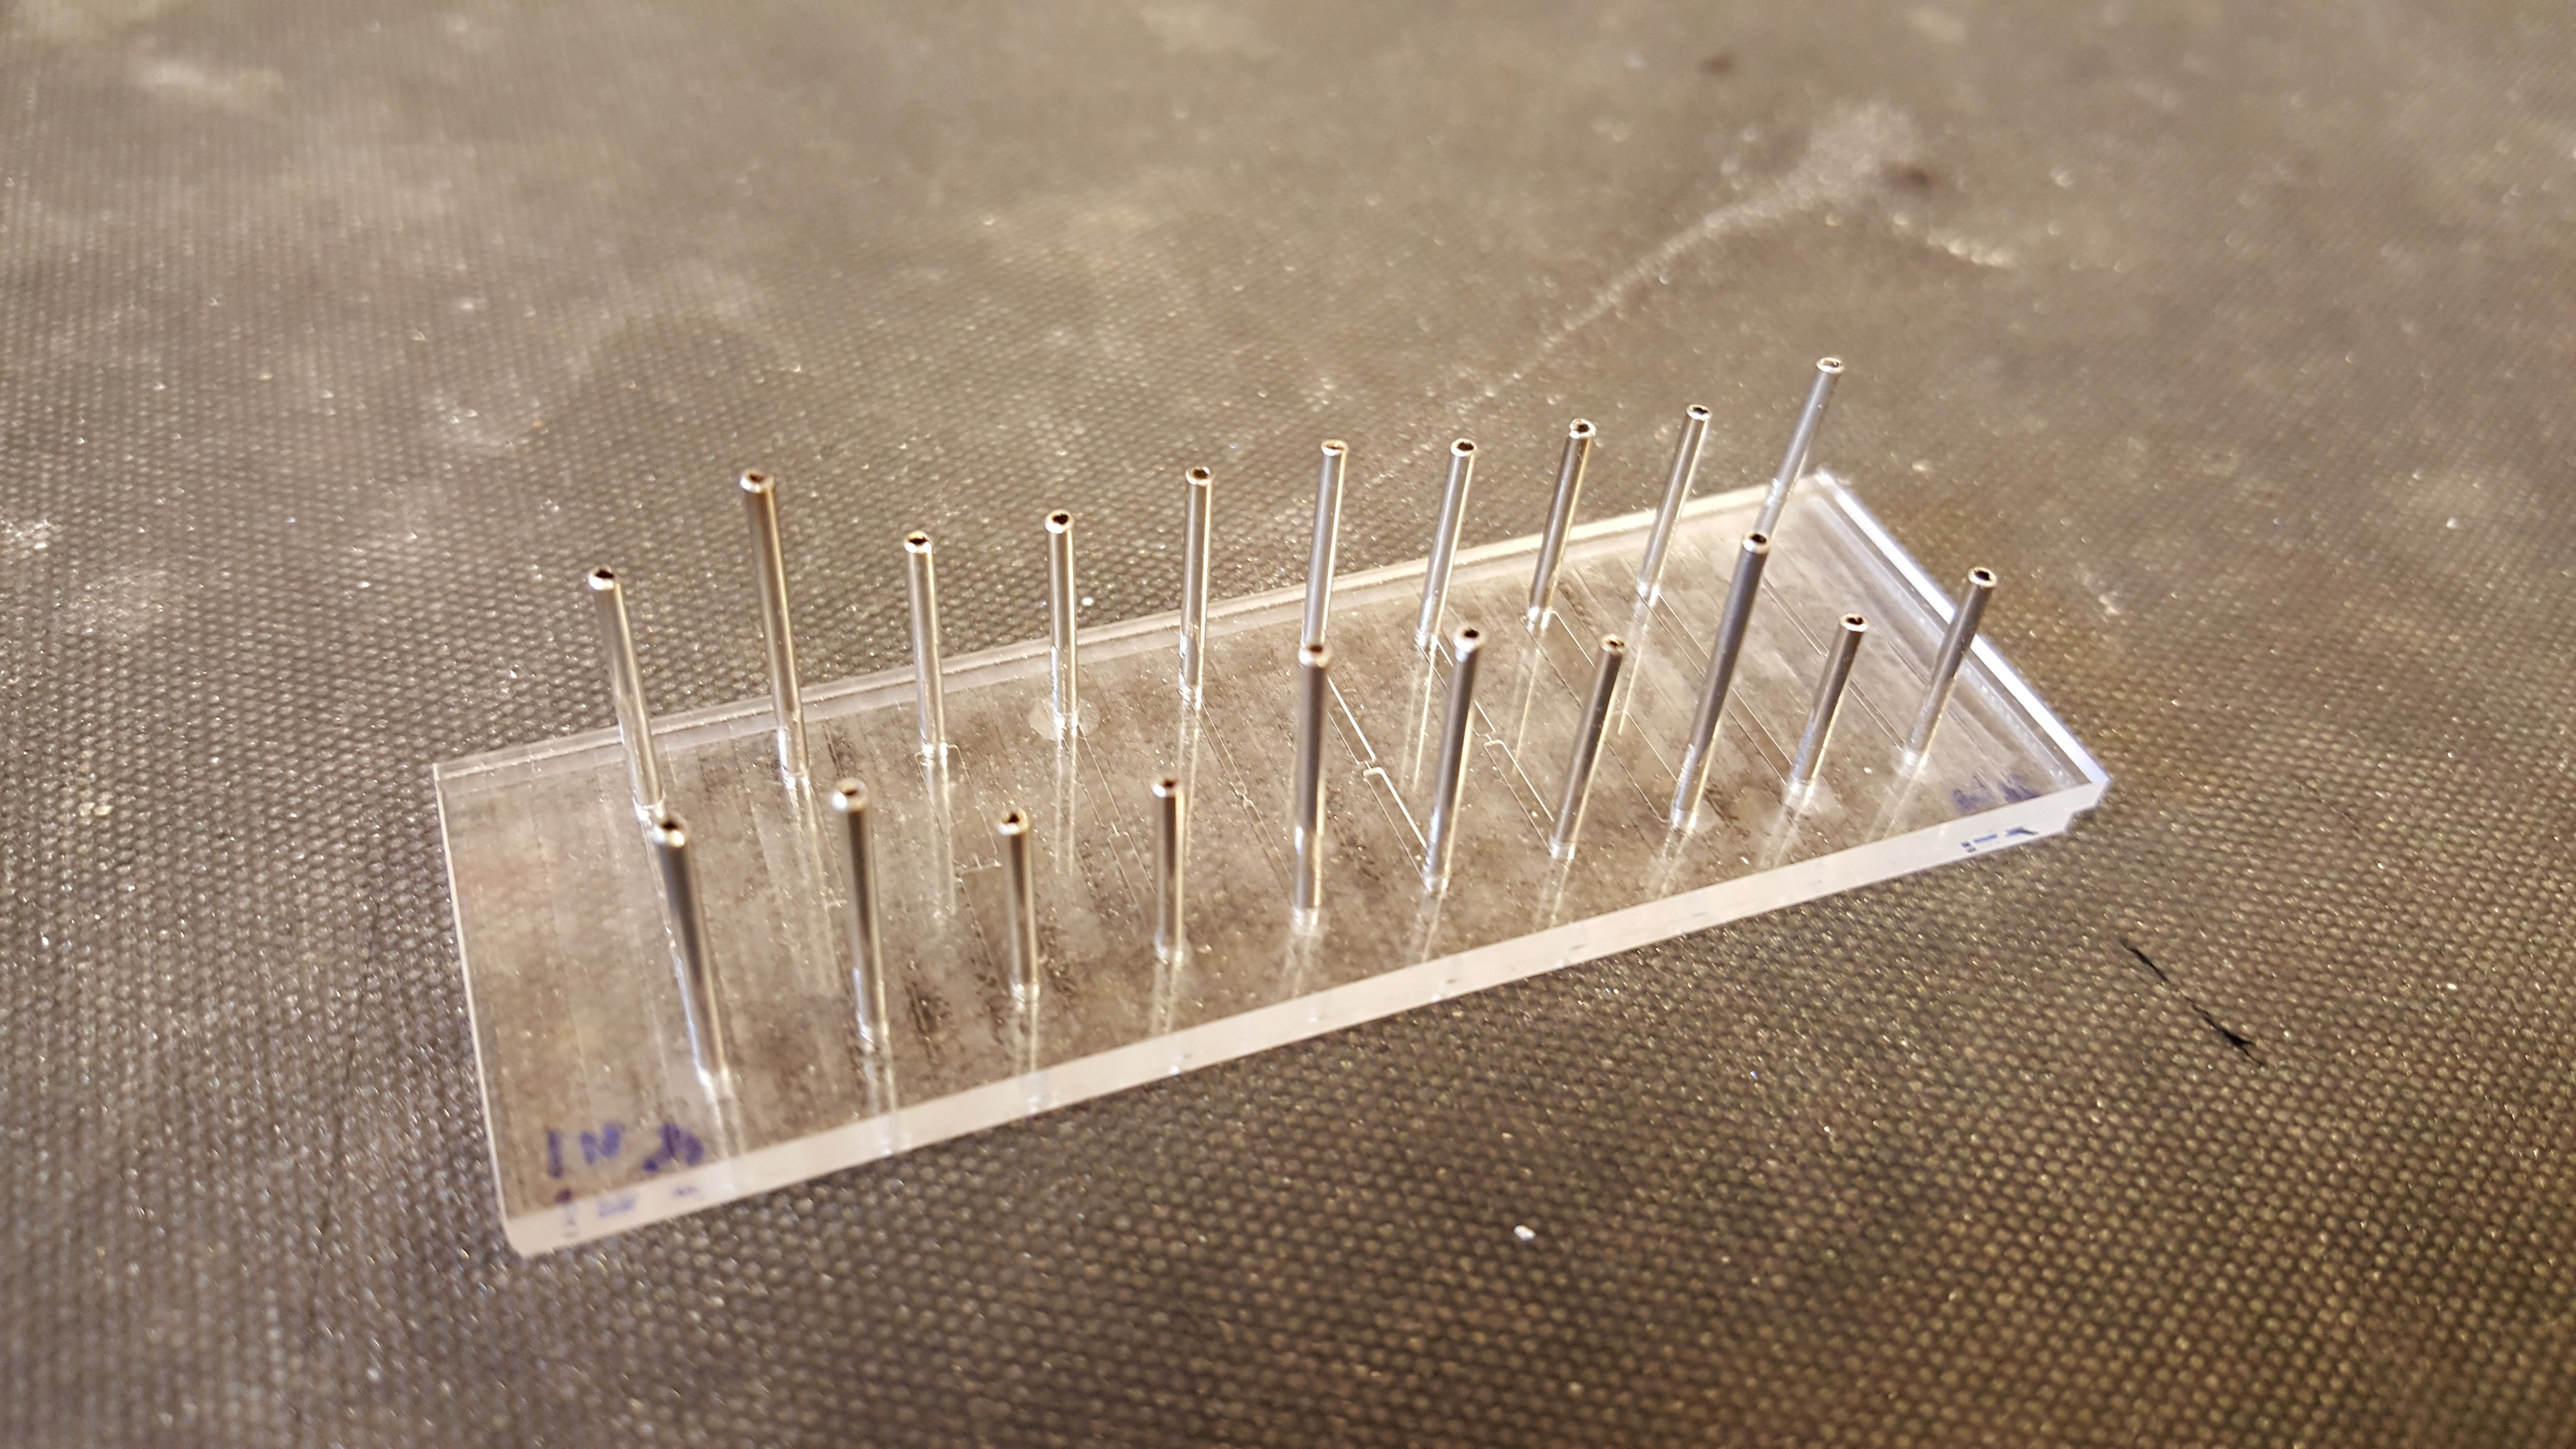
\includegraphics[width=0.5\textwidth]{finalchip.png}
		\caption{\label{fig:chip} Final sample on PMMA sheet with two channels for each dimension. Channel 1, 2, 3, 4, 5, etc. Steel tubes were inserted at inlets and outlets for easy coupling.}
        	\end{center}
\end{figure}
 
Detailed images of the final chips' constricted sections of all channels are seen in Fig.~\ref{fig:1channel} throughout Fig.~\ref{fig:5channel}.

\begin{figure}
\begin{center}
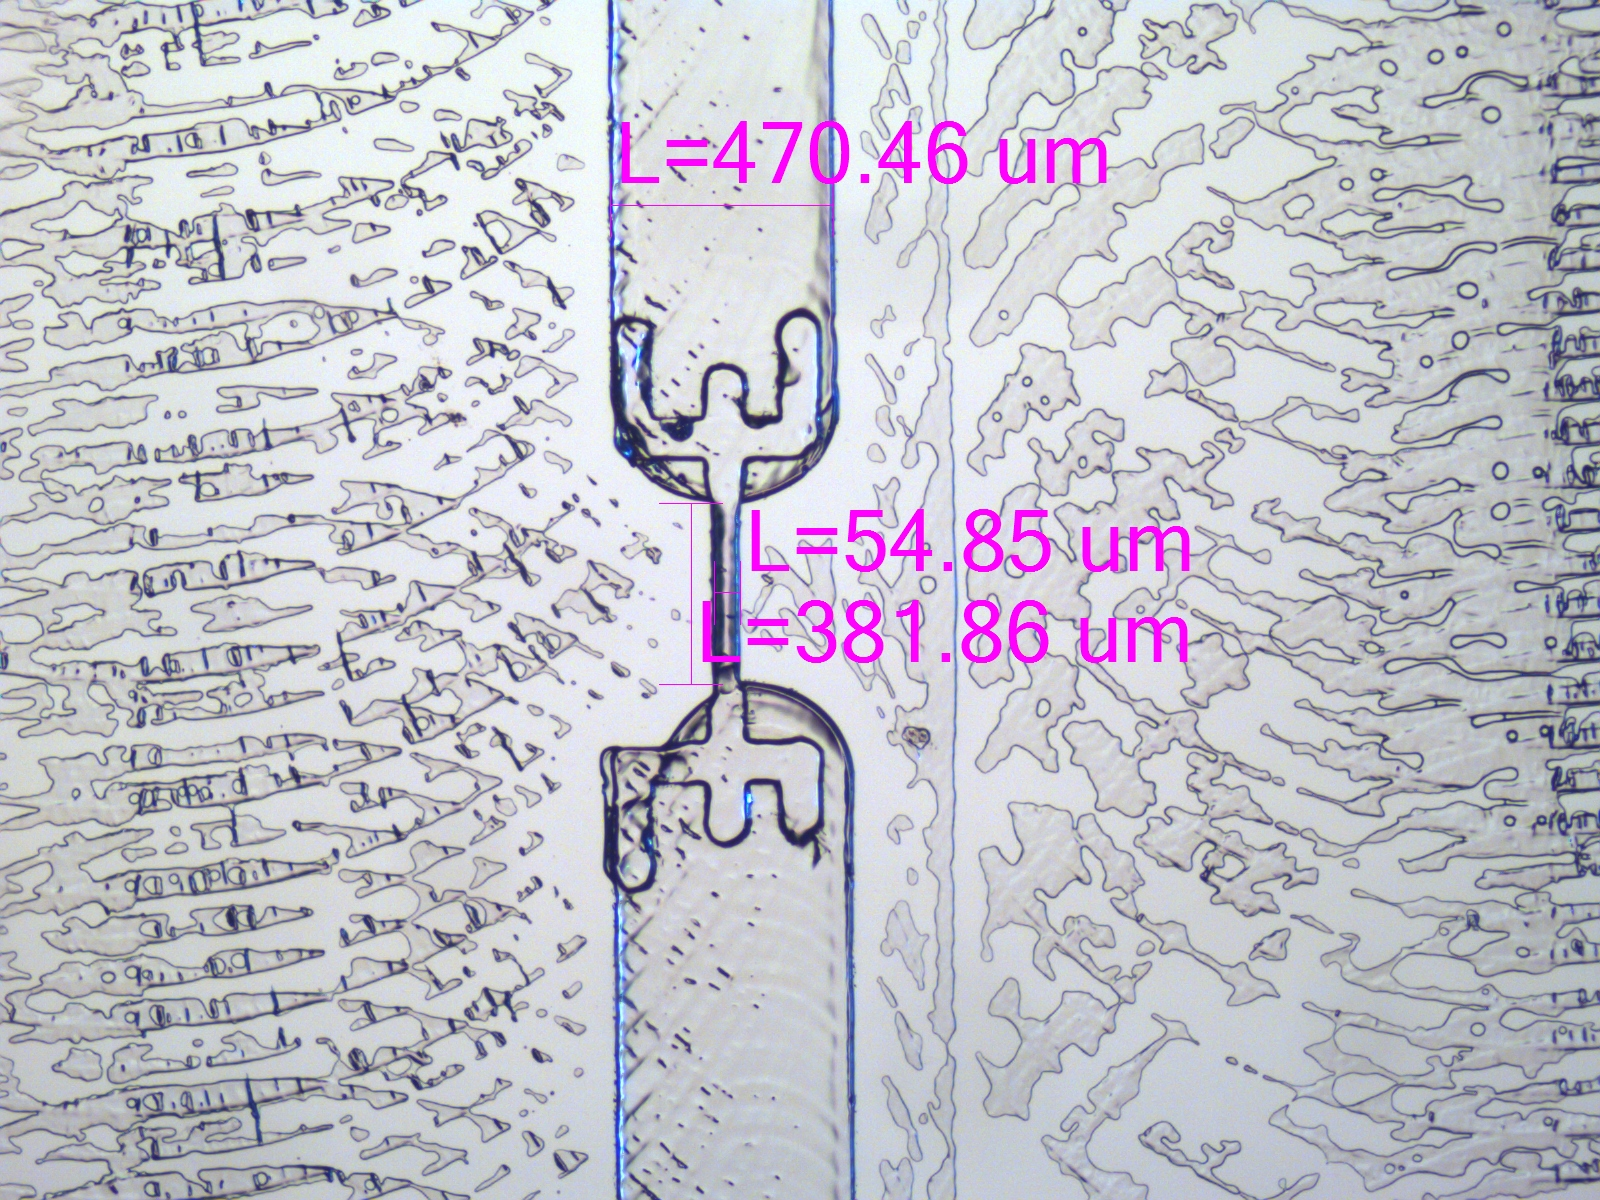
\includegraphics[width=0.5\textwidth]{w500d100Dim.jpg}
		\caption{\label{fig:1channel} Close up of channel 1. Width 500 $\mu$m, depth 100 $\mu$m.}
        \end{center}
\end{figure}

\begin{figure}
\begin{center}
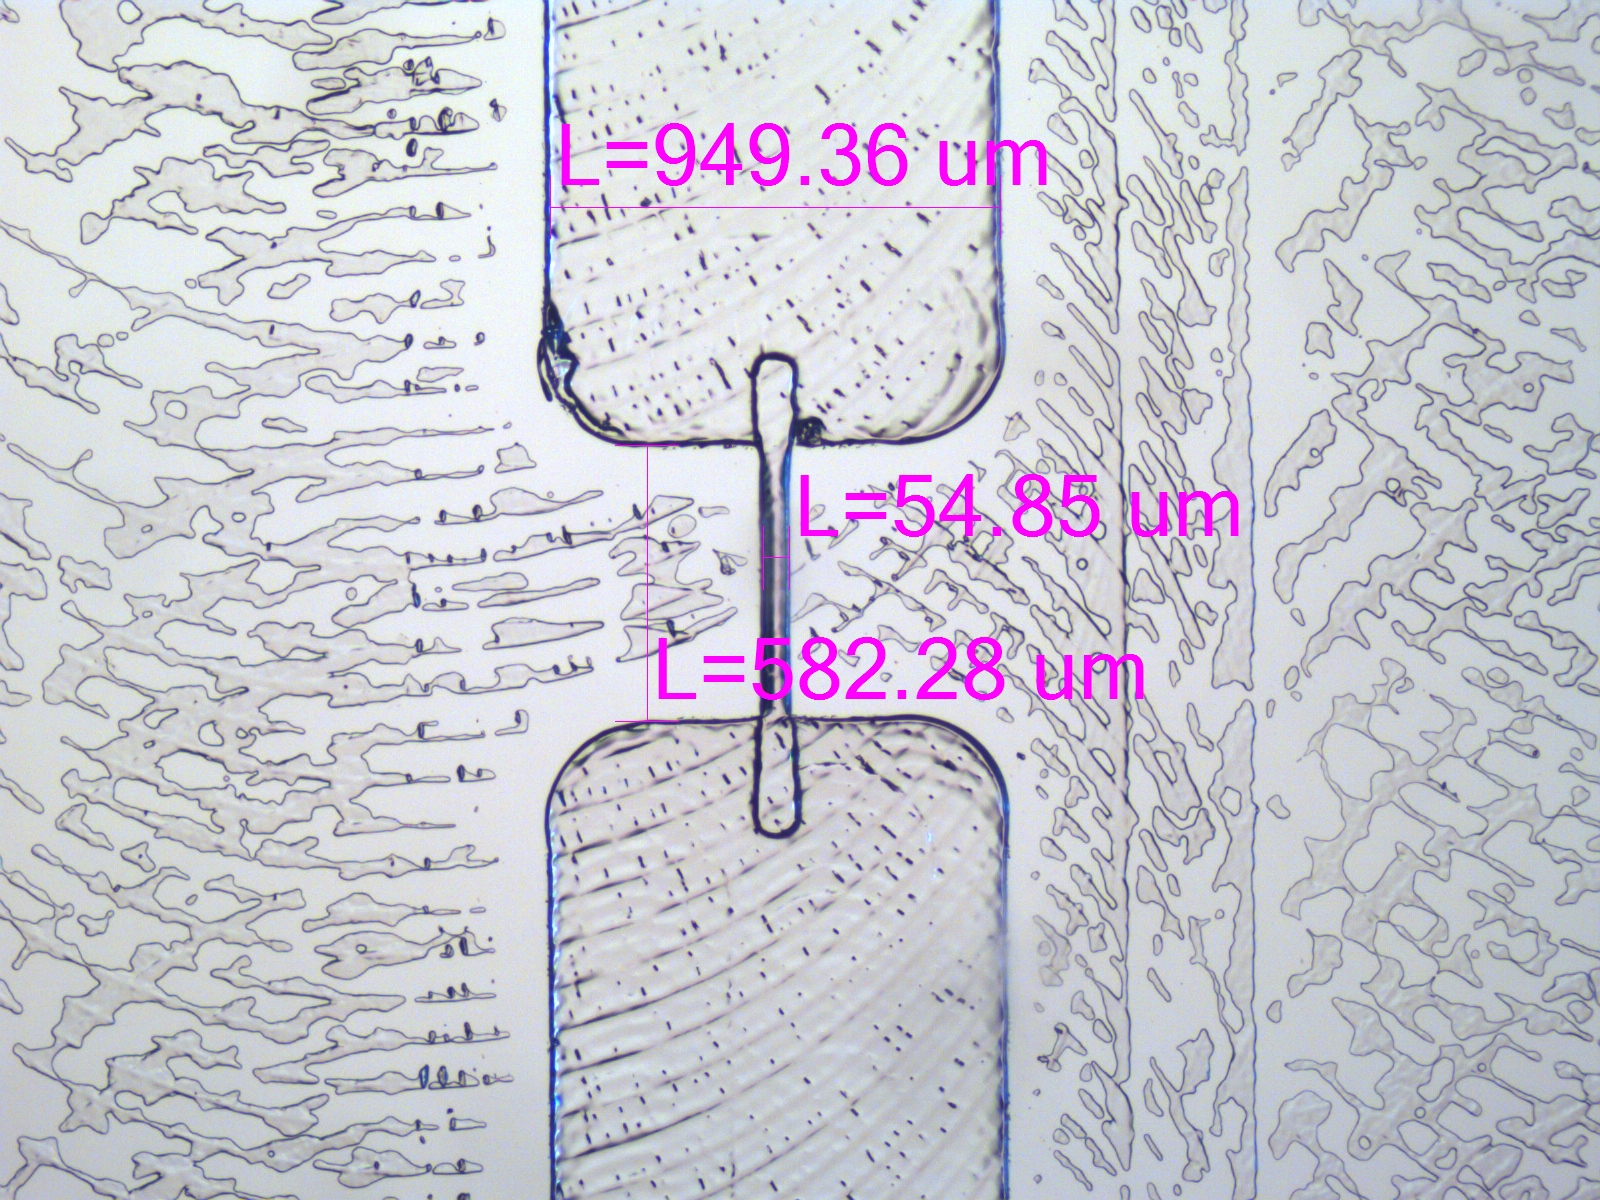
\includegraphics[width=0.5\textwidth]{w1000d100Dim.jpg}
		\caption{\label{fig:2channel} Close up of channel 2. Width 1000 $\mu$m, depth 100 $\mu$m.}
        \end{center}
\end{figure}
    
\begin{figure}
\begin{center}
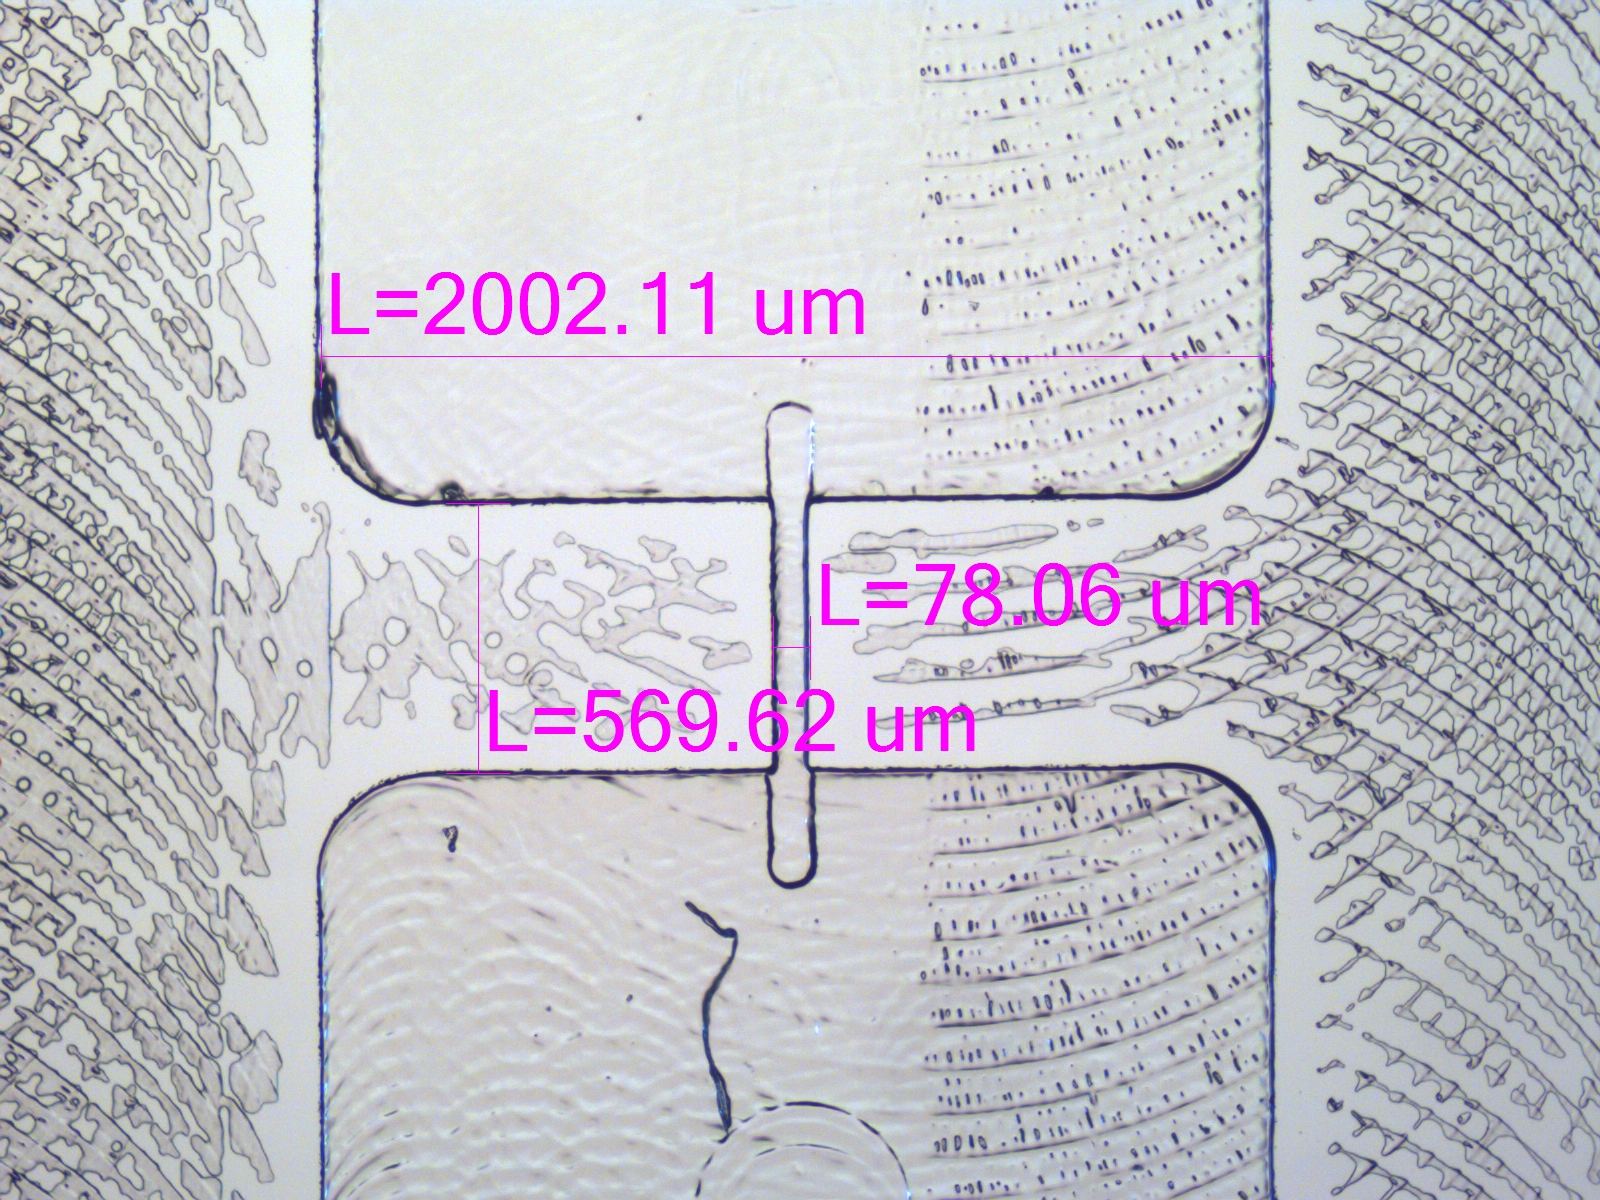
\includegraphics[width=0.5\textwidth]{w2000d100Dim.jpg}
		\caption{\label{fig:3channel} Close up of channel 3. Width 2000 $\mu$m, depth 100 $\mu$m.}
        \end{center}
\end{figure}

\begin{figure}
\begin{center}
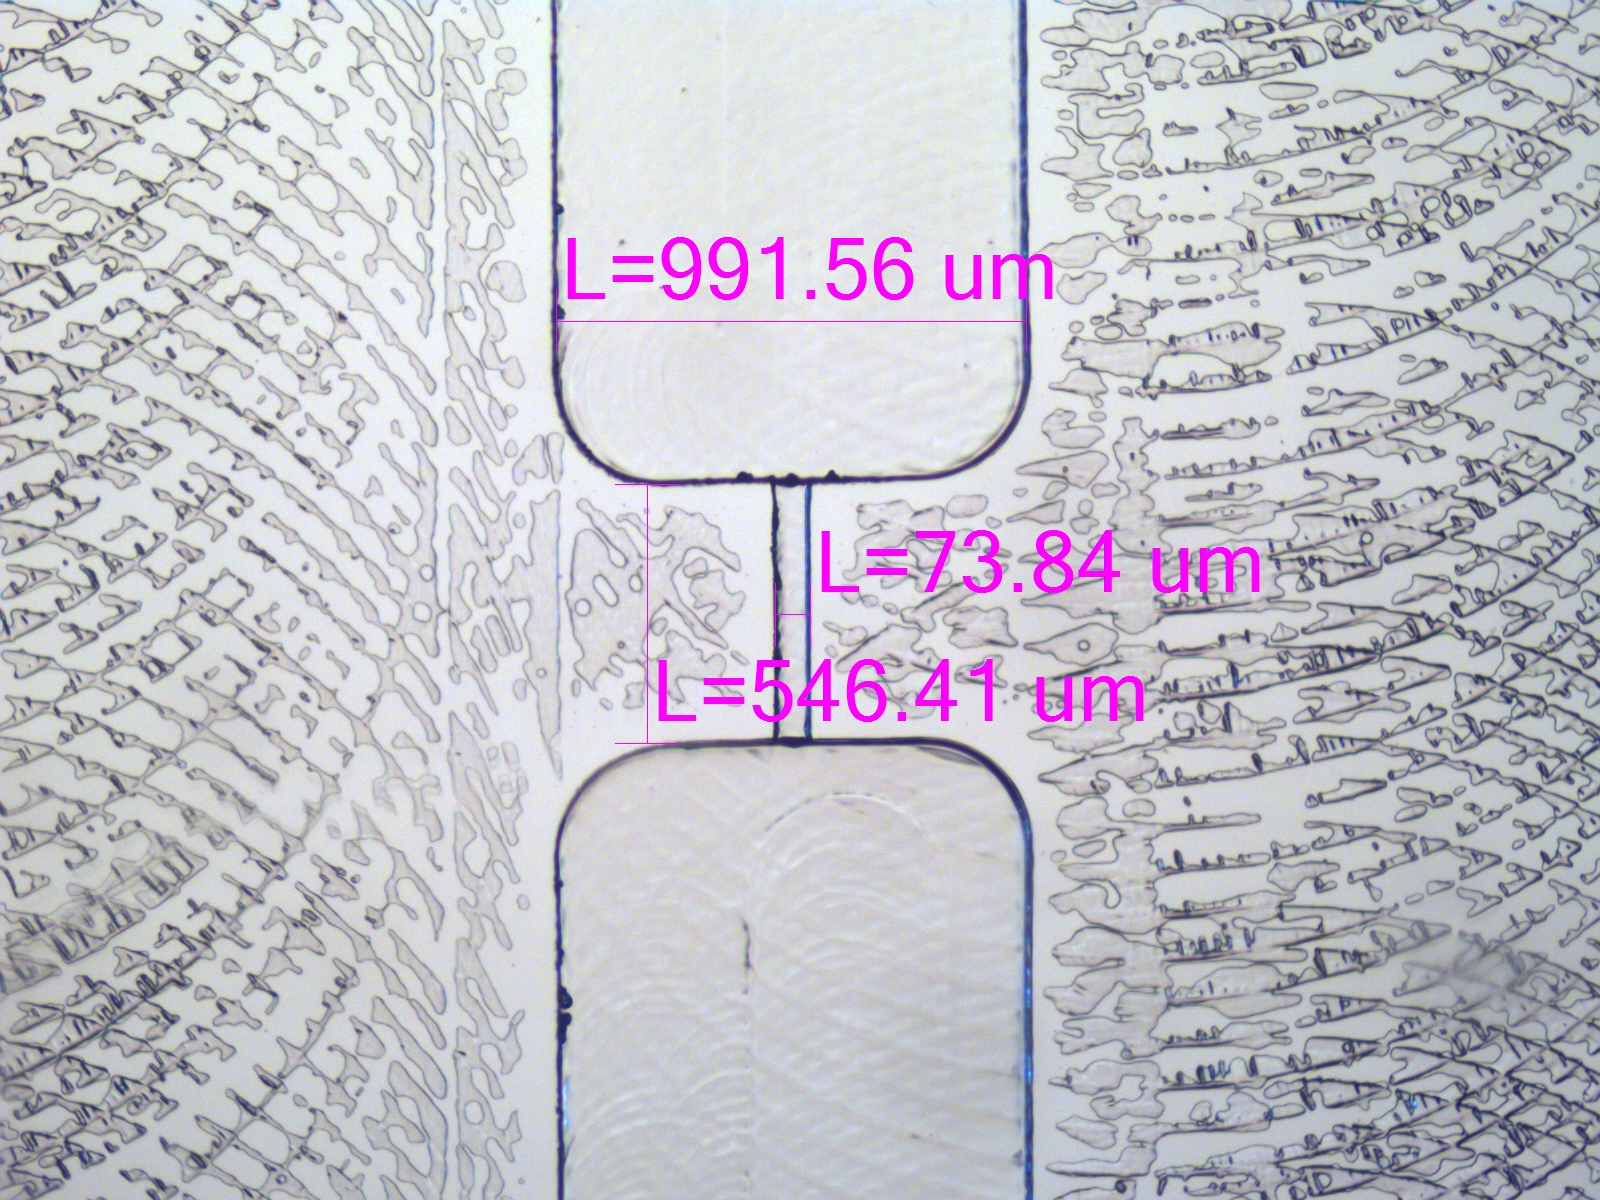
\includegraphics[width=0.5\textwidth]{w1000d200Dim.jpg}
		\caption{\label{fig:4channel} Close up of channel 4. Width 1000 $\mu$m, depth 200 $\mu$m.}
        \end{center}
\end{figure}
    
\begin{figure}
\begin{center}
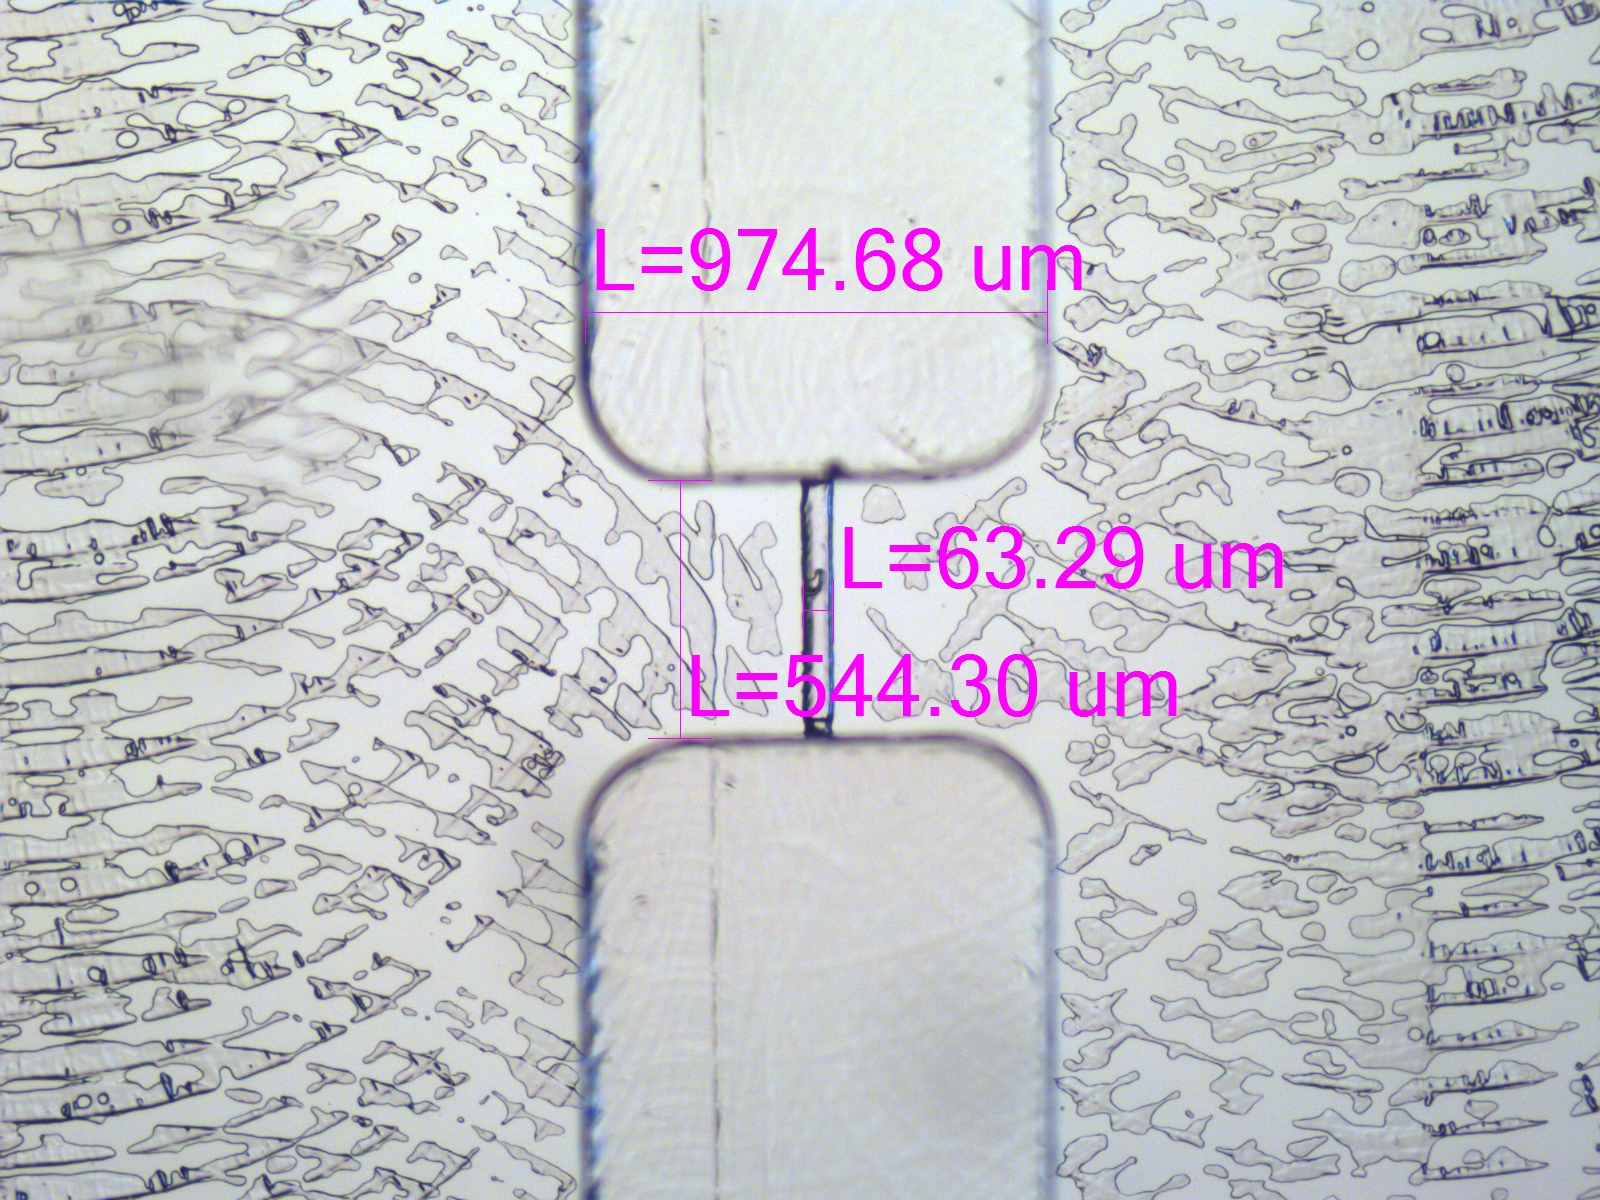
\includegraphics[width=0.5\textwidth]{w1000d400Dim.jpg}
		\caption{\label{fig:5channel} Close up of channel 5. Width 1000 $\mu$m, depth 400 $\mu$m.}
        \end{center}
	\end{figure}

\subsection{Trapping}
The chip was placed under a microscope, and the channel of interest was continuously displayed on an adjacent screen. Electrodes were attached to the tubing at the inlet and outlet of the channel being tested, and connected to a voltage source. The first attempt to identify an iDEP effect was done in the 3D-channels, assuming they were most likely to have a large enough constriction ratio to trap the particles efficiently. In order to cleanse the channel of contaminating particles, fibres and air bubbles before each iDEP attempt, the channels were washed with water mixed with 1\% PBS. A identical mix, with a small amount of TWEEN added, was used as the test sample, with a conductivity of approximately 100 $\mu$S. The properties of the PBS were in accordance with what have been presented in literature for successful iDEP experiments, aiming to acquire a Clausius-Mossotti factor of -0.5 and thus creating an n-DEP force \cite{Braff:12}.

A PBS mixture with 0.1\% Tween, with 12 $\mu$m polystyrene particles mixed were used. The particle mixture was injected in the channels, the system was made to rest and able to reach ''steady state'' and then the voltage source was turned on at around 20-25 V. Gradually the voltage was increased until a trapping effect was observed. An upper limit on the current was set to 0.25 mA in order to avoid excessive heating. To ensure sufficient contact between the electrodes and the liquid in the channels silver threads were inserted in the pipes at each channel end, and the electrodes were directly attached to these instead. 

In order to change the operating conditions and investigate the impact of the channel media, a solution of 100\% PBS with 8$\mu$m polystyrene particles were mixed with the previously used diluted PBS solution, creating a final PBS concentration of approximately 50\%. The solution started to boil and the channel was filled with bubbles immediately when the voltage was turned on.
   
\section{Results \& discussion}

\subsection{FEM simulations}
The simulations of the electric potential and field lines are seen in Fig~\ref{fig:potField}. The increase of electric field concentration is seen just to the left and right of the constricted part of the channel.
\begin{figure}[!hbt]
	\begin{center}
		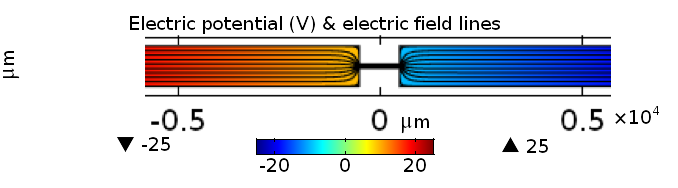
\includegraphics[width=\columnwidth]{potFieldW1000d100_new.png}
		\caption{\label{fig:potField} Electric potential and field lines of a 2D model with the dimensions of channel 2 (Table~\ref{tab:dim}). Inlet of the channel is on the left.}
	\end{center}
\end{figure}

The simulations shows what is to be expected and no unexpected phenomena were observed.

\subsection{Fabrication}
In Fig-~\ref{fig:1channel} throughout Fig.~\ref{fig:5channel} the results from the fabrication is seen close up. In channel 1 a severe defect is observed around the constriction section, which is probably due to wrongly coded paths and depths for the micro milling process. Some residual particles and fibers are observed in the images and distinct traces from the cutting tool are observed as well. The sheets were not fully bonded which resulted in cavities (darker areas) but it is also clear that these are not present near the walls in any of the channels. This means that they do hold tight. It should be mentioned that the width of the constricted section was well below the 100 $\mu$m that was sketched up in all channels, which is probably a result of the bonding process.

\subsection{Trapping}
The trapping in the channels at different voltages is visible in Fig.~\ref{fig:1-50V} 
through Fig.~\ref{fig:3-76V} below. The red circles in the microphotos encircles where the trapping effect is most dominant and clearly visible.

Trapping for different voltages applied to channel 1 is observed in Fig.~\ref{fig:1-50V} and Fig.~\ref{fig:1-96V}.

\begin{figure}[!hbt]
	\begin{center}
		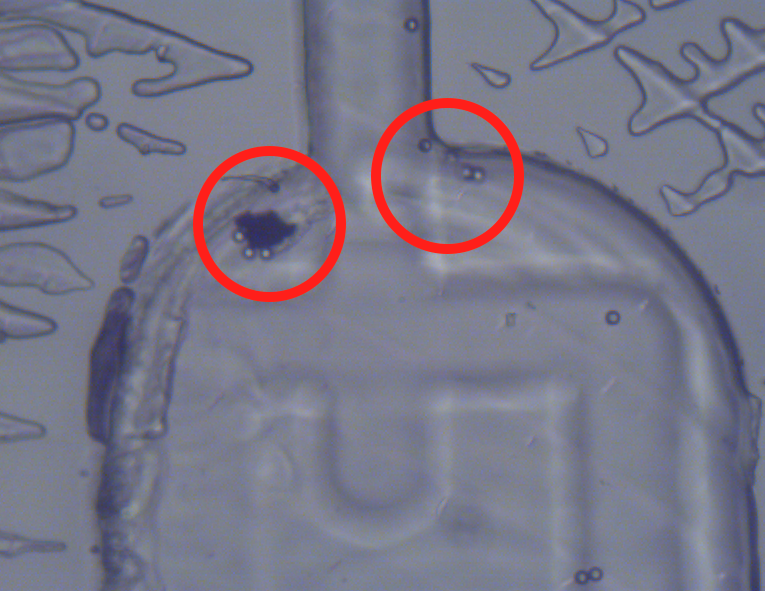
\includegraphics[width=\columnwidth]{1-50V.png}
		\caption{\label{fig:1-50V} Trapping of 12 $\mu$m particles at 50V in channel 1. The red circles shows where the trapping effect occurs.}
	\end{center}
\end{figure}

\begin{figure}[!hbt]
	\begin{center}
		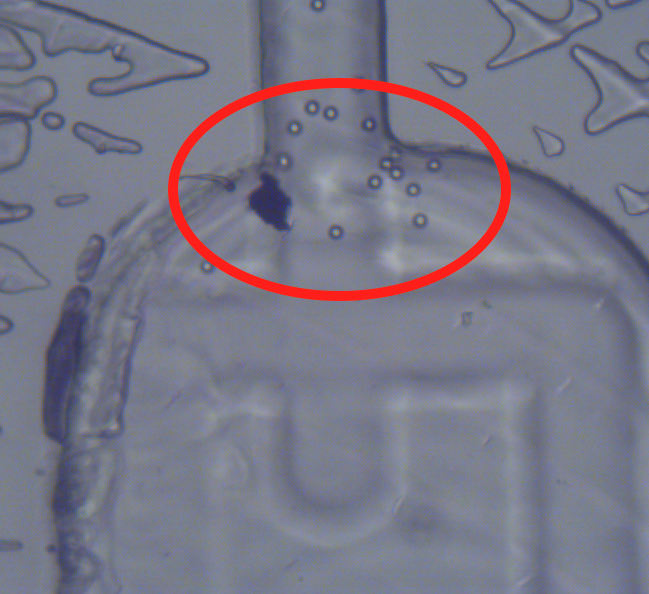
\includegraphics[width=\columnwidth]{1-96V.png}
		\caption{\label{fig:1-96V} Trapping of 12 $\mu$m particles at 96V in channel 1. The red circle shows where the trapping effect occurs.}
	\end{center}
\end{figure}

Trapping in channel 4 at 102 V is observed in Fig.~\ref{fig:4-102V}.

\begin{figure}[!hbt]
	\begin{center}
		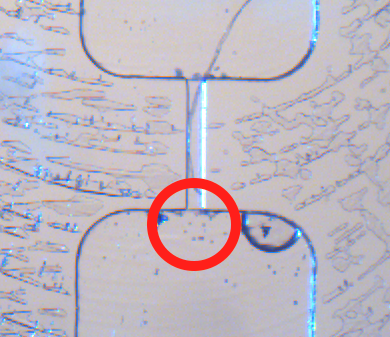
\includegraphics[width=\columnwidth]{4-102V.png}
		\caption{\label{fig:4-102V} Trapping of 12 $\mu$m particles at 102V in channel 4. RThe red circle shows where the trapping effect occurs.}
	\end{center}
\end{figure}

The trapping effect in channel 3 at 76 V is observed in Fig.~\ref{fig:3-76V}.
\begin{figure}[!hbt]
	\begin{center}
		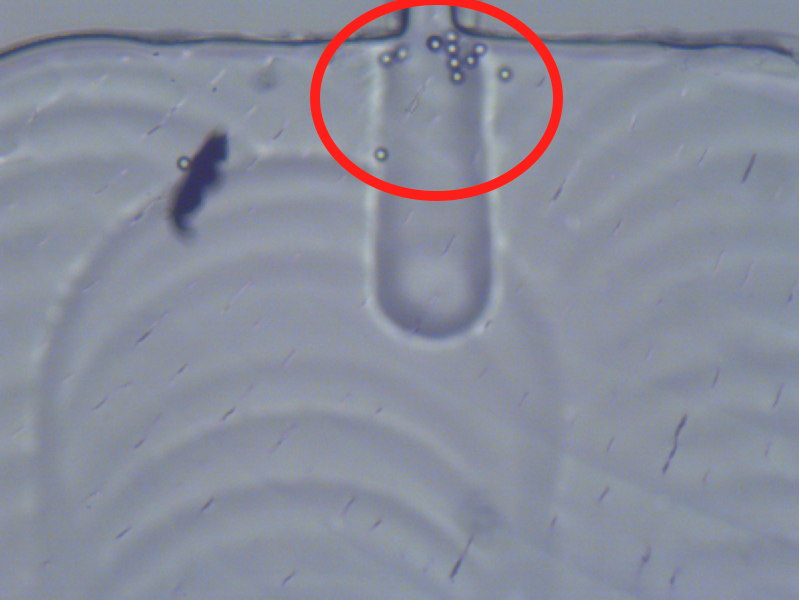
\includegraphics[width=\columnwidth]{3-76V.png}
		\caption{\label{fig:3-76V} Trapping of 12 $\mu$m particles at 76V in channel 3. The red circle shows where the trapping effect occurs.}
	\end{center}
\end{figure}

\section{Conclusion}

The first particles with 8 $\mu$m in diameter were tested were definitely too numerous to serve the purpose of iDEP trapping, as they quickly became indistinguishable and clustered.
For the 12 $\mu$m particles, the electroosmotic flow induced movement of the particles from $+$ to $-$ when voltage was applied, and trapping was visible in all channels but at different voltages. The lowest potential at which trapping could be identified was in channel 1 (final constriction ratio 8) at 50 V. This was unexpected, since this was the channel with the lowest constriction ratio. Overall, channel 1 performed trapping just as well as (if not better than) the channels with larger constriction ratios at equal voltages.
In the other channels, sedimentation before reaching the constricted part was more of an issue and thus the applied potential needed to be increased above 50 V before enough particles reached the constricted area and trapping could occur. In general for the other channels, trapping started to occur at around 60V, and particle velocity and trapping strength increased as the voltage increased up to 110 V. The exact relationship between voltage and trapping strength is though hard to confirm with our results. Neither could a significant difference in trapping strength between the 2D and 3D channels be confirmed. The 3D channels had constriction ratios of 20 and 40, but we could not conclude that channel 5 trapped twice as well as channel 4 at equal voltages, nor better than channel 1 or 2, which had significantly lower constriction ratios. This also applied for the 2D channels, where channel 2 (constriction ratio 10) and channel 3 (constriction ratio 20) performed equally at the same voltage. More attempts with each channel dimension would be needed in order to draw such conclusions. 
A reason for the lack of trapping intensity in the 3D channels could be due to that not as many particles reached the constricted area due to the ‘depth step’ in those channels. Many particles moving along the bottom of the channel are likely to not reach up to the constricted part, due to rather slow flow rates. It is likely that they sedimented instead, as sedimentation was more frequently occurring in the 3D channels. This could be considered a drawback with this method, considering that if high potentials are required in order to reach sufficient flow rates, these are associated with undesired heating effects.  
When the electric field was turned off, particle movement as well as trapping ceased. This indicates that the trapping that was detected at least is coupled to the electric field, and not just turbulence at the entrance of the constricted channel.

Considering that this was our first model of an iDEP device, being able to trap particles is a small success. However, we were not able to quantify the trapping and quantify our results. For future iDEP projects, we suggest that other geometries are investigated as well as larger particle sizes and particles with altered dielectric properties. More trials for each insulating geometry is also necessary. Clean PBS should not be used as a fluid since heat production quickly becomes an issue. The greatest challenge is how to quantify the results. In order to quantify the importance of the constriction ratio, a suggestion is that constriction ratios of greater difference are compared, e.g. 10 vs. 100 or greater. In this project the greatest difference was eightfold (between 5 and 40 in theory, and after the bonding maybe higher) and during our operating conditions, no significant difference between their trapping abilities could be observed.

Altogether, we believe that the simplicity of an iDEP device is a great advantage, and that it has a future especially in biological applications, as it, if applied correctly, could be an efficient way of handling heat sensitive samples.

%Bibliography section.
\bibliographystyle{ieeetr}
\bibliography{reference}
% Your document ends here!
\end{document}